\chapter{Multi-version Execution}
\label{chap:multi-version}

An indisputable and widely accepted fact is that all software contains bugs.
These bugs cause software failures which can lead to anything from minor
discomfort and loss of service to major disasters including loss of lives.
Software reliability is the probability of failure-free operation for specified
period of time in a specified environment.

There are two basic approaches to increase software reliability. One is fault
avoidance, using formal specification and verification methods, and a rigorous
software development process. Another approach is fault tolerance, through
replication, redundancy and diversity. Two popular software fault tolerance
methods that use diversity are $N$-version programming~\cite{avizienis:nvp} and
recovery block~\cite{randell:rb}.

%$N$-version programming (NVP) has been first introduced in 1970's as a way to
%increase reliability of software by having independent teams to design and
%implement the same functionality multiple times from the same specification as
%different program versions. 

The idea behind $N$-version programming (NVP) is to have independent teams to
design and implement the same functionality multiple times from the same
specification as different program versions. These versions are then run in
parallel using an $N$-version execution environment (NVX) and their results are
voted on and the majority of the outputs is selected.

$N$-version programming depends on the assumption that software errors in
different versions are independent. Otherwise, these versions are not effective
at detecting errors as the different versions are likely to contain the same
bugs. The experiment done by Knight and Leveson~\cite{knight86,knight90} shown
that the assumption of independence does not hold and independently developed
versions had the same or similar software faults 50\% of the time in more than
one version since programmers tended to commit certain classes of mistakes
dependently.

Despite the criticism, $N$-version programming is still widely accepted as an
effective technique for improving reliability. The problem is that even small
probability of correlated bugs in different version significantly reduces the
potential reliability improvement, which makes the $N$-version programming less
cost-effective compared to other fault-tolerance due to a need for developing
$N$ different version. Lui Sha~\cite{lui01} compared different fault tolerance
approaches and suggested that, assuming finite software development cycle, it
is better to invest resources into a single reliable implementation rather than
three different implementations which will be run in parallel.

The issue of cost related to development of multiple independent versions has
been partially addressed by the multi-variant program execution, which can be seen
as an evolution of $N$-version programming. Rather than developing different versions
of the same application manually, these are generated from a single version
using different techniques such as special source code
annotations~\cite{onlinevalidation,trachsel10}, code transformations based on
the modification of the abstract syntax tree~\cite{schulte14,sosie:issta14},
custom compilers producing different binary layout for different
variants~\cite{orchestra09,unibus:nspw10}. %, or even specialized runtime
%environments which customize different aspects of application runtime
%state~\cite{diehard06,tightlip}.

Rather than executing $N$ different versions of the same program, we could also
run different programs where one program acts as a specification and other
implementations are checked against the specification at runtime.  This is the
basic idea behind runtime monitoring and checking~\cite{kim:mac,java-mac01}. In
runtime monitoring and checking, one program is the implementation while
another is the specification. The implementation is checked against the
specification at runtime, which is easier than proving the equivalence
statically (or formally).  Furthemore, the specification can be less efficient
and thus simple. The example shown by Lui Sha in~\cite{lui01} uses Bubblesort
as a runtime specification for Quicksort.

%However, Hatton~\cite{hatton97} argued that even dependent $N$-version
%programming provides significant reliability improvement and it is therefore
%more cost-effective to develop $N$ average versions rather than one good
%version.

\section{Software updates}

% Recent years have seen a growing interest in using diversity as a way to
% increase the reliability and security of software systems.  One form of
% software diversity that has attracted significant interest from the research
% community is the idea of running multiple diversified versions of a program in
% parallel in order to survive bugs and detect security attacks.  In essence,
% diversity can offer probabilistic guarantees that at least one variant survives
% a bug, or that a security attack will be flagged by divergent behaviour across
% variants.

% On the reliability side, which forms the main focus of this thesis, these
% diversified versions are either automatically-generated variants, multiple
% versions of the same application, or different programs implementing the same
% interface.  For example, one may run in parallel multiple variants that employ
% complementary thread schedules to survive concurrency
% errors~\cite{compl-schedules11}, multiple versions of the same software to
% survive update bugs~\cite{mx}, or multiple web browsers to benefit from the
% fact that many errors do not affect all browser
% implementations~\cite{cocktail}.  In this thesis, we show that running multiple
% versions in parallel can be used in other reliability scenarios, such as
% running expensive error detectors (``sanitizers'') during deployment.

% On the security side, these diversified variants are constructed in such a way
% as to reduce the probability of an attack succeeding in all of
% them~\cite{cox2006,orchestra09,diehard06,tightlip,capizzi08,devries10,cocktail,trachsel10}.
% For example, one may generate versions with a different arrangement of memory
% blocks in the address space~\cite{diehard06}, or with stacks growing in
% opposite directions~\cite{orchestra09}, to prevent attacks whose success
% depends on the memory layout.

One particularly important class of bugs are bugs introduced by software
updates. These bugs often affect existing functionality, degrading the
reliability, and potentially also security, of the software. This leads to
frustration as users are no longer able to use the functionality they have been
able to use in the past; as a consequence, users often refuse applying updates
to their software and rely instead on outdated versions, which may contain bugs
and security vulnerabilities.

To address this problem, we propose a variant of $N$-version execution focused
on improving reliability and availability of updated software:
\emph{multi-version execution}.  While $N$-version execution and multi-version
execution techniques have many similarities, there are several key differences.
First and foremost, in $N$-version execution the different version are
developed by different teams while multi-version execution uses the consequent
revisions, which are product of natural software evolution. Second, the goal of
$N$-version execution is increasing the reliability of software by running
independently developed, functionally equivalent software variants, whereas
multi-version assumes that the variants are largely the same except for parts
affected by the software update.

While designed primarily in the context of software updates, the multi-version
execution technique can be applied in many different scenarios, including
$N$-version execution. Furthermore, as shown in this thesis, multi-version
execution runtimes can be used in other reliability scenarios, such as running
expensive error detectors (``sanitizers'') during deployment or implementation
of security honeypots.

% There are two key differences between our proposed approach and
% previous work in this space.  First, we do not rely on automatically
% generated variants, but instead propose to use existing software
% versions as a mechanism for improving software updates.  This also
% means that as opposed to previous solutions, the versions running in
% parallel are not semantically equivalent---this eliminates the
% challenge of generating diversified variants and creates opportunities
% in terms of recovery from failures, but also introduces additional
% challenges in terms of synchronising the execution of the different
% versions.  Second, while previous work has focused on detecting
% divergences, our key concern is to \textit{survive} them,
% in order to increase the reliability, availability, and security 
% of the overall application.

% Running different versions of an application in parallel has been used
% to test and validate software patches.  Tachyon~\cite{tachyon12} is an
% online patch testing system in which the old and the new version of an
% application are run concurrently; 
% when a divergence is detected, the options are to either halt the
% program, or to create a manual rewrite rule specifying how to handle
% the divergence.  Delta execution~\cite{onlinevalidation} similarly
% uses two different versions of a single application, splitting the
% execution at points where the two versions differ, and comparing their
% results to test the patch for errors and validate its
% functionality.  
% By comparison, the focus of this proposal is on ``managing'' such
% divergences at runtime in order to keep the application running, and
% therefore runtime deployment and crash recovery play a central role in
% our approach.

% Research on surviving software failures has received a lot of
% attention in the
% past~\cite{rx,compl-schedules11,fo,exec-trans06,vigilante,clearview,microreboots},
% and our proposed approach can benefit from the techniques developed in
% this context.  Compared to this prior work, the main novelty lies in
% combining multiple software versions to survive failures.

\section{Real-world scenarios}
\label{multi-version:scenarios}

To motivate the multi-version execution technique, we present three existing
scenarios involving the \vim editor, as well as \lighttpd, and \redis servers.
These correspond to two categories of applications that could benefit from our
approach: user applications such as text editors for which reliability is a key
concern; and network servers, with stringent security and availability
requirements.

% To motivate the multi-version execution technique, we present several existing
% scenarios involving the \chrome browser and the \vim editor, as well as the
% \lighttpd, \redis and \vsftpd servers. These correspond to two categories of
% applications that could benefit from our approach: desktop applications such as
% web browsers and office tools for which reliability is a key concern; and
% network servers, with stringent security and dependability requirements.

% \gchrome\footnote{\url{http://www.google.com/chrome}} is one of the most widely
% used web browsers.  Even though \chrome releases are tested extensively before
% deployment, they sometimes introduce new bugs that affect the stability of the
% browser.  A concrete example is version $6.0.466.0$, which introduced a bug
% that caused \chrome to crash when trying to load certain web pages over
% SSL.\footnote{\url{http://code.google.com/p/chromium/issues/detail?id=49197}}
% One might argue that in this case the user should downgrade to an older version
% and wait until the bug is fixed. However, versions immediately preceding
% $6.0.466.0$ suffer from a different
% bug,\footnote{\url{http://code.google.com/p/chromium/issues/detail?id=49721}}
% which was introduced in version $6.0.438.0$ and which crashes Chrome during
% certain sequences of repeated back and forward navigation.

% \vim\footnote{\url{http://www.vim.org/}} is arguably one of the most popular
% text editors.  In version $7.1.127$, while trying to fix a memory leak,
% \vim developers introduced a double \textstt{free} bug that caused \vim to
% crash whenever the user tried to use a path completion feature.  This bug made
% its way into \textit{Ubuntu} $8.04$, affecting a large number of
% users.\footnote{\url{https://bugs.launchpad.net/ubuntu/+source/vim/+bug/219546}}

% \lighttpd\footnote{\url{http://www.lighttpd.net/}} is a popular web-server used
% by several high-traffic websites such as Wikipedia and Xkcd.
% Despite its popularity, crash bugs are still a common
% occurrence in \lighttpd, as evident from its bug tracking
% database.\footnote{\url{http://redmine.lighttpd.net/issues/}}
% As one example, a patch introduced in April
% 2009\footnote{\url{http://redmine.lighttpd.net/projects/lighttpd/repository/revisions/2438}}
% (correctly) fixed the way HTTP ETags are computed.
% Unfortunately, this fix broke the support for compression, which relied on the
% previous way in which ETags were computed and resulted in a segmentation fault
% whenever a client requested HTTP compression.  This issue was only diagnosed
% and reported in March
% 2010\footnote{\url{http://redmine.lighttpd.net/issues/2169}} and fixed at the
% end of April
% 2010,\footnote{\url{http://redmine.lighttpd.net/projects/lighttpd/repository/revisions/2723}}
% more than one year after it was introduced, leaving the server vulnerable to
% possible attacks in between.

% \redis is an advanced key-value data structure
% server,\footnote{\url{http://redis.io/}} often referred to as one the most
% popular NoSQL databases.  Due to its performance and low-resource requirements,
% \redis is being used by many well-known services such as GitHub.  Because the
% whole dataset is held in memory, reliability is critically important, as a
% crash could result in total data loss.  However, like any other large software
% system, \redis is subject to crash bugs. Issue
% 344\footnote{\url{http://code.google.com/p/redis/issues/detail?id=344}} is one
% such example.  This issue causes \redis to crash when the \textstt{HMGET}
% command is used with the wrong type. The bug was introduced in April 2010,
% diagnosed and reported only half a year later in October 2010 and then fixed
% after fifteen days.

% \vsftpd\footnote{\url{https://security.appspot.com/vsftpd.html}} is a fast and 
% secure FTP server for UNIX systems.  Version $2.2.0$ added several new
% features such as network isolation, but unfortunately also introduced
% a bug\footnote{\url{https://bugs.launchpad.net/ubuntu/+source/vsftpd/+bug/462749}}
% which triggered a segmentation fault whenever a client used the
% passive FTP mode.  This bug made \vsftpd practically unusable since
% the passive mode is being frequently used by clients behind firewalls.
% Despite being reported several times, this bug was only fixed in
% version $2.2.1$, released more than two months after the bug was
% introduced.

\subsection{\vim double free error on home path completion}

\vim\footnote{\url{http://www.vim.org/}} is arguably one of the most popular
text editors. While trying to fix a memory leak, \vim developers introduced a
double \lstinline`free` bug that caused \vim to crash whenever the user tried to
use a path completion feature. This bug was introduced in version 7.1.127,
released in September 2007. The incorrectly fixed version of the
\lstinline`ExpandOne` function is shown in Listing~\ref{lst:vim-bug}. The newly
introduced code frees up the memory used to store the expanded path.
Unfortunately, when the path contains the \lstinline`~` symbol used as an alias for
user's home directory, this code path will be invoked twice leading to a crash.

\begin{lstlisting}[alsolanguage=diff,numbers=none,label=lst:vim-bug,caption={First (incorrect) fix of \lstinline`ExpandOne` function in \vim.}]
@@ -3543,0 +3548,4 @@ ExpandOne(xp, str, orig, options, mode)
+    /* Free "orig" if it wasn't stored in "orig_save". */
+    if (orig != orig_save)
+       vim_free(orig);
+
\end{lstlisting}

The double \lstinline`free` bug was detected and fixed in version 7.1.147, released
one month later in October 2007. The correct version of the \lstinline`ExpandOne`
function is shown in Listing~\ref{lst:vim-fixed}. In this version, the
\lstinline`orig_saved` variable type was changed to \lstinline`int` and is
being used as a flag preventing the second \lstinline`free` invocation.

\begin{lstlisting}[alsolanguage=diff,numbers=none,label=lst:vim-fixed,caption={Second (correct) fix \lstinline`ExpandOne` function in \vim.}]
@@ -3355,0 +3356 @@ ExpandOne(xp, str, orig, options, mode)
+    int                orig_saved = FALSE;
@@ -3423,0 +3425 @@ ExpandOne(xp, str, orig, options, mode)
+       orig_saved = TRUE;
@@ -3549 +3551 @@ ExpandOne(xp, str, orig, options, mode)
-    if (orig != orig_save)
+    if (!orig_saved)
        vim_free(orig);
\end{lstlisting}

Despite the bug being fixed promptly, it made its way into Ubuntu 8.04,
affecting a large number of
users.\footnote{\url{https://bugs.launchpad.net/ubuntu/+source/vim/+bug/219546}}
Since the 8.04 is a long-term support version, the Ubuntu maintainers avoid
incorporating new changes except for critical security bug fixes. This meant
that the \vim users affected by this bug had to build and install their own
version of \vim from the source.

\subsection{\lighttpd mod\_compress segfault with disabled ETag support}

\lighttpd\footnote{\url{http://www.lighttpd.net/}} is a popular open-source 
web-server used either alone or in conjunction with other web-servers
by several high-traffic websites such as Wikipedia and Xkcd.
Despite its popularity, crash bugs are still a common
occurrence in \lighttpd, as evident from its bug tracking
database.\footnote{\url{http://redmine.lighttpd.net/issues/}}  Below
we discuss one such bug, which our approach could successfully
eliminate.

In April 2009, a patch was
applied\footnote{\url{http://redmine.lighttpd.net/projects/lighttpd/repository/revisions/2438}}
to \lighttpd's code related to the HTTP ETag functionality.  An ETag
is a unique string assigned by a web server to a specific version of a
web resource, which can be used to quickly determine if the resource
has changed.  The patch was a one-line change, which discarded the
terminating zero when computing a hash representing the ETag.  More
exactly, line 47 in \textstt{etag.c}:

\begin{lstlisting}[numbers=none,breaklines=true,xleftmargin=0pt]
for (h=0, i=0; i < etag->used; ++i) h = (h<<5)^(h>>27)^(etag->ptr[i]);
\end{lstlisting}
\noindent was changed to:
\begin{lstlisting}[numbers=none,breaklines=true,xleftmargin=0pt]
for (h=0, i=0; i < etag->used@-1@; ++i) h = (h<<5)^(h>>27)^(etag->ptr[i]);
\end{lstlisting}

This correctly changed the way ETags are computed, but unfortunately,
it broke the support for compression, whose implementation depended on
the previous computation.  More precisely, \lighttpd's support for HTTP
compression uses caching to avoid re-compressing files which have not
changed since the last access.  To determine whether the cached
file is still valid, \lighttpd internally uses ETags.  Unfortunately,
the code implementing HTTP compression did not consider the case when
ETags are disabled.  In this case, \textstt{etags->used}
is \textstt{0}, and when the line above is
executed, \textstt{etag->used-1} underflows to a very large value, and
the code crashes while accessing \textstt{etag->ptr[i]}.
Interestingly enough, the original code was still buggy (it always
returns zero as the hash value, and thus it would never re-compress
the files), but it was not vulnerable to a crash.

The segfault was diagnosed and reported in March
2010\footnote{\url{http://redmine.lighttpd.net/issues/2169}} and fixed
at the end of April
2010,\footnote{\url{http://redmine.lighttpd.net/projects/lighttpd/repository/revisions/2723}}
more than one year after it was introduced.  
%The history is depicted graphically in Figure~\ref{fig:lighttpd-history}.  
% The bottom line is
% that for about one year, users affected by this buggy patch
% essentially had to decide between%
% \begin{inparaenum}[(1)]
% \item incorporating security and bug fixes added to the code, but being
%   vulnerable to this crash bug, and
% \item giving up on these security and bug fixes and using an old version of
%   \lighttpd, which is not vulnerable to this bug.
% \end{inparaenum}
% Note that this is particularly true for the eleven-month period
% between the time when the bug was introduced and the time it was
% diagnosed, since during this period most users would not know how to
% change the server's configuration to avoid the crash.

%% The original code, which can be seen in Listing~\ref{lst:2437}, makes the
%% \texttt{i < etag->used} comparison (line 4). Because both \texttt{i} and
%% \texttt{etag->used} are $0$, the condition \texttt{0 < 0} does not hold and
%% the loop body will never be executed.

%% The affected code can be seen in Listing~\ref{lst:2438}. Here, the condition
%% has been changed and comparison has now the form \texttt{i < etag->used-1}.
%% When executing, the \texttt{etag->used} variable will underflow and condition
%% \texttt{0 < 4294967295} will be true. Therefore, the loop body will be
%% executed and access to \texttt{etag->ptr[0]} will result in segmentation
%% fault.

\subsection{\redis crash on wrong \textstt{HMGET} type}

\begin{figure}[t]
\begin{minipage}[b]{0.90\columnwidth}
\begin{lstlisting}[label=lst:original, caption={Original (correct) version of the {\footnotesize \texttt{hmgetCommand}} function in \redis.}]
robj *o = lookupKeyRead(c->db, c->argv[1]); /*@\label{line:key-found}@*/
if (o == NULL) {
  addReplySds(c,sdscatprintf(sdsempty(),"*%d\r\n",c->argc-2));
  for (i = 2; i < c->argc; i++) {
    addReply(c,shared.nullbulk);
  }
  return;
} else {
  if (o->type != REDIS_HASH) { /*@\label{line:type-found}@*/
    addReply(c,shared.wrongtypeerr); /*@\label{line:report-error}@*/
    return; /*@\label{line:return}@*/
  }
}
addReplySds(c,sdscatprintf(sdsempty(),"*%d\r\n",c->argc-2));
\end{lstlisting}
\end{minipage}
\hspace{2.2\columnsep}
\begin{minipage}[b]{0.9\columnwidth}
\begin{lstlisting}[label=lst:refactored, caption={Refactored (buggy) version of the {\footnotesize \texttt{hmgetCommand}} function in \redis.}]
robj *o, *value;
o = lookupKeyRead(c->db,c->argv[1]);
if (o != NULL && o->type != REDIS_HASH) {
  addReply(c,shared.wrongtypeerr); /*@\label{line:report-error2}@*/
}
addReplySds(c,sdscatprintf(sdsempty(),"*%d\r\n",c->argc-2));
for (i = 2; i < c->argc; i++) {
  if (o != NULL && (value = hashGet(o,c->argv[i])) != NULL) { /*@\label{line:hashGet}@*/
    addReplyBulk(c,value);
    decrRefCount(value);
  } else {
    addReply(c,shared.nullbulk);
  }
}
\end{lstlisting}
\end{minipage}
\end{figure}

\redis is an advanced key-value data structure
server,\footnote{\url{http://redis.io/}} often referred to as one the most
popular NoSQL databases.  Due to its performance and low-resource requirements,
\redis is being used by many well-known services such as GitHub.  Because the
whole dataset is held in memory, reliability is critically important, as a
crash could result in total data loss.  However, like any other large software
system, \redis is subject to crash bugs. Issue
344\footnote{\url{http://code.google.com/p/redis/issues/detail?id=344}} is one
such example.  This issue causes \redis to crash when the \textstt{HMGET}
command is used with the wrong type.  The bug was introduced during a code
refactoring applied in revision \textstt{7fb16bac}.  The original code of the
problematic \textstt{hmgetCommand} function is shown in
Listing~\ref{lst:original}, while the (buggy) refactored version is shown in
Listing~\ref{lst:refactored}.

In the original code, if the lookup on line~\ref{line:key-found} is successful,
but the type is not \textstt{REDIS\_HASH} (line~\ref{line:type-found}), the
function returns after reporting an incorrect type
(lines~\ref{line:report-error}--\ref{line:return}). However, in the refactored
version (Listing~\ref{lst:refactored}), the \textstt{return} statement is
missing, and after reporting an incorrect type (line~\ref{line:report-error2}),
the function continues execution and causes segmentation fault inside the
\textstt{hashGet} function invoked on line~\ref{line:hashGet}. This is a
critical bug, which may result in losing some or even all of the stored data in
case when the Append Only File (AOF) persistence log is corrupted due to issue
620\footnote{\url{http://code.google.com/p/redis/issues/detail?id=620}}.

The bug was introduced in April 2010, diagnosed and reported only half a year
later in October 2010 and then fixed after fifteen days.  As in the case of the
\lighttpd bug, this means that for several months, any \redis instance was
susceptible to a crash and vulnerable to a possible attack.


\section{Parallel software execution}

% All the scenarios presented above describe software updates which, while trying
% to fix existing bugs or refactor the code, also introduced new bugs that caused
% the code to crash under certain conditions. Improving the reliability of such
% updates is the main goal of our proposed approach: running both the old and the
% new version in parallel after an update can enable applications to survive more
% errors, without giving up the new features introduced by the update.

% The bottom line for all the presented scenarios is that for significant amount
% of time, \ie about one year in case of \lighttpd and six months in case of
% \redis, users affected by buggy patches essentially had to decide between%
% \begin{inparaenum}[(1)]
% \item incorporating other security and bug fixes added to the code, but being
%   vulnerable to these crash bug, and
% \item giving up on these security and bug fixes and using an old version of
%   \lighttpd or \redis, which are not vulnerable to these newly introduced bugs.
% \end{inparaenum}
% Note that this is particularly true for the period between the time when the
% bug was introduced and the time it was diagnosed (\ie eleven months in case of
% \lighttpd, six months in case of \redis), since during this period most users
% would not know how to change the server's configuration to avoid the crash.

All the scenarios presented above describe software updates which, while trying
to fix existing bugs or refactor the code, also introduced new bugs that caused
the code to crash under certain conditions. The bottom line for all these
scenarios is that for significant amount of time, \ie about one year in case of
\lighttpd and six months in case of \redis, users affected by buggy patches
essentially had to decide between%
\begin{inparaenum}[(1)]
\item incorporating other security and bug fixes added to the code, but being
  vulnerable to these crash bug, and
\item giving up on these security and bug fixes and using an old version of
  \lighttpd or \redis, which are not vulnerable to these newly introduced bugs.
\end{inparaenum}
Note that this is particularly true for the period between the time when the
bug was introduced and the time it was diagnosed (\ie eleven months in case of
\lighttpd, six months in case of \redis), since during this period most users
would not know how to change the server's configuration to avoid the crash.

Our approach aims to provide users with a third choice; when a new version
arrives, instead of replacing the old version, we will run both. The goal
of our approach is to run multiple versions of an application in parallel, and
synchronize their executions so that%
\begin{inparaenum}[(1)]
\item users are given the illusion that they interact with a single version of
  the application,
\item the multi-version application is at least as reliable and secure as any
  of the individual versions in isolation, and
\item the synchronization mechanism incurs a reasonable performance overhead.
\end{inparaenum}

As shown in Figure~\ref{fig:mx-platform}, our solution requires a form of
virtualization framework that would coordinate the execution of multiple
application versions, and mediate their interaction with the external
environment. Various such frameworks have been designed in the past in the
context of running multiple automatically generated variants of a given
application in parallel~\cite{diehard06,cox2006,orchestra09}, and many of the
techniques proposed in prior work can be reused in our context.  To be
practical, this coordination mechanism has to incur a reasonable overhead on
top of native execution and ensure that the overall system is able to scale up
and down the number of software versions run in parallel in order to balance
conflicting requirements such as performance, reliability, security and energy
consumption.

\begin{figure}[t]
  \begin{center}
    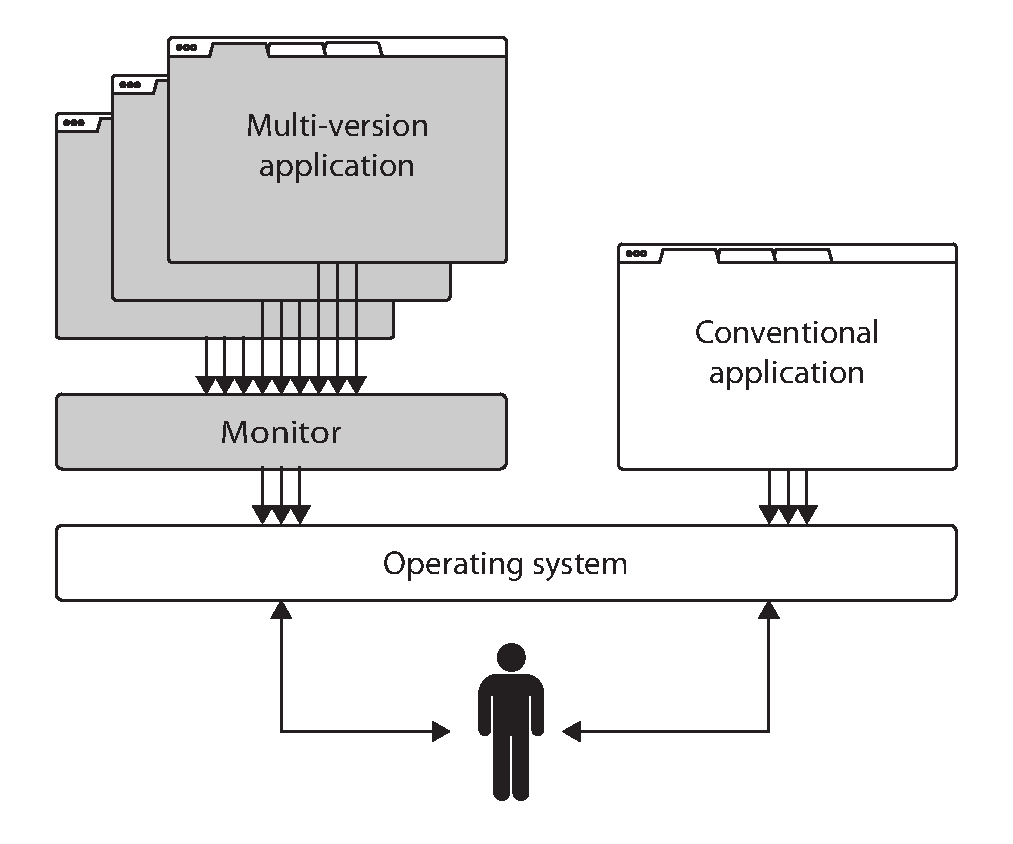
\includegraphics[width=0.5\textwidth]{multi-version/figures/platform}
    \caption{A platform running conventional and multi-version
      applications side by side.}
    \label{fig:mx-platform}
  \end{center}
\end{figure}

One particular challenge for our approach is to detect any divergences between
different software versions, resolve them in such a way as to increase the
overall reliability of the application, and finally synchronize again the
different versions after their executions reconverge to the same behavior.  Of
course, we also need to handle the case in which the executions of different
versions fail to reconverge to the same behavior after sufficient time.

Selecting the ``correct'' behavior of an application when different versions
disagree is of course not possible in the general case without having access to
a high-level specification.  However, one could%
\begin{inparaenum}[(1)]
\item focus on universal
correctness properties, such as the absence of crashes, and
\item use various
heuristics such as majority voting and favoring the latest application
versions.
\end{inparaenum}
Our approach is to resolve a divergence by always using the behavior of the
version that has not crashed, and favoring the behavior of the latest version
in all other cases. In this way, we ensure that the overall application has
strictly fewer crashes than any of the individual versions, while still using
the new security and bug fixes implemented in the latest version.

% Note that one key aspect on which our approach relies is
% \textit{having the different versions be alive at all times}.  This ensures
% that applications can survive crashes that occur at different points
% in different versions, but adds the extra challenge of restarting
% crashed versions.

%% Once divergences are detected, we need to decide what output should be
%% selected as the output of the multi-version system in order to improve
%% overall reliability.  Many different strategies can be used, but the
%% common goal is to ensure that the multi-version system will have
%% strictly fewer errors than any of the individual versions.

% Finally, our approach needs a deployment strategy to decide what versions are
% run in parallel when the number of available resources (\eg, idle CPU cores) is
% limited.  We envision several options---such as keeping the last $N$ released
% versions (where $N$ is the number of available resources), or keeping several
% very old stable versions---but the exact strategy should be decided on a
% case-by-case basis. % using existing empirical data.

\section{Challenges}

There are several different ways to implement an effective system call monitor,
each with its own set of trade-offs. The solutions targeting binaries are
significantly easier to use---they can be typically applied to off-the-shelf
binaries---but compared to solutions operating at source code level, they give
up some of the precision while typically require more engineering effort. The
most common ways for implementing monitors operating on binaries are dynamic
linking, \ptrace, kernel extensions and binary instrumentation, while solutions
targeting source code typically rely on source code instrumentation.

System calls are rarely performed directly by the application, which rather use
the wrapper functions provided by the C library. By linking to a custom
library, which provides a custom version of these functions, we could intercept
system calls performed by the application. This could be done either statically
at link time~\cite{plash}, or dynamically at runtime~\cite{shepherding:pldi14}
(\eg using \lstinline`LD_PRELOAD` or \lstinline`DYLD_INSERT_LIBRARIES`
variables). The major benefit of this approach is efficiency and relative ease
of implementation. However, the mechanism could be easily bypassed (\eg by
invoking system calls directly); also the C library ABI is has significantly
larger surface compared to the system call interface, requiring more
engineering effort.

\ptrace is an interface provided by most UNIX-like operating systems, including
Linux, providing means by which a process might observe and control another
process. The primary use of \ptrace interface is for debugging, but the
relative ease of use makes \ptrace a popular choice for implementing system
system call monitors~\cite{wily-hacker,orchestra09,tachyon12}. \ptrace-based
solutions require relatively low engineering effort, which makes them
especially suitable for rapid prototyping~\cite{spillane07}, they are easy to
deploy and fairly flexible. On the other hand, the use of \ptrace has numerous
drawbacks: a significant performance overhead due to large number of context
switches, problematic support for multi-threaded applications, and the lack of
filtering mechanism allowing interception only of system calls of interest.
\ptrace-based solution are also more difficult to debug as the use of \ptrace
disallows the use of \ptrace-based debuggers such as \gdb.

% The performance overhead could be partially improved by the use of
% more efficient mechanism for copying memory from/to the monitored process, such
% as shared memory as in case of Orchestra~\cite{orchestra09}, or cross memory
% attach as in case of \mx (\S\ref{sec:mxm}). The lack of filtering mechanism
% could be addressed by combining \ptrace with \textsf{seccomp/bpf} mechanism as
% shown by \textsc{Mbox}~\cite{mbox}.

An alternative to \ptrace is to implement the system call monitor
entirely~\cite{provos2002,cox2006} or partially in kernel space~\cite{ostia}.
While this approach has numerous advantages compared to other approaches, such
as minimal performance overhead and direct access to the application's
execution context and address space, there are several drawbacks.  First, this
approach requires kernel patches and/or new new kernel modules which
complicates the development, limits portability across different operating
systems or even different kernel versions, and hinders maintainability. Second,
the monitor must be run in privileged mode, which means that bugs in the
implementation may compromise the system stability. Furthermore, it also makes
it difficult for regular users to deploy and use such monitors.

Binary rewriting technique allow transforming the executable (either statically
or dynamically) altering its functionality; as such, it can be used to
implement system call monitor by rewriting all system call instructions into a
control flow transfer instructions (\eg a
\lstinline[language={[x64]Assembler}]`jmp` instruction). Existing monitors were
built either on top of existing binary rewriting
systems~\cite{onlinevalidation}, or using a purpose built binary translation
mechanism~\cite{vx32}. The advantage of binary rewriting-based monitors is
relatively low performance overhead, especially in the case of purpose built
rewriting mechanism. The main disadvantage is the complexity of implementation
which requires significant development effort.

In this thesis, we present two different designs for building monitors suitable
for multi-version execution. The first one, called \varan described in
Chapter~\ref{chap:efficient-execution}, is aimed towards running large number
of versions side-by-side with low performance overhead, and uses selective
binary rewriting to achieve this goal. The second one, called \mx described in
Chapter~\ref{chap:safe-updates}, is focused on surviving crashes caused by bugs
introduced in software updates, with the prototype implementation built using
the \ptrace mechanism.

%%%%%%%%%%%%%%%%%%%%%%%%%%%%%%%%%%%%%%%%%%%%%%%%%%%%%%%%%%%%%%%%%%%%%%%%%%%%%%

% Our approach aims to provide users with a third choice; when a new version
% arrives, instead of replacing the old version, we run both versions in
% parallel. In our example, consider that we are using \mx to run a
% version of \lighttpd from March 2009.  When the buggy April 2010 version
% is released, \mx runs it in parallel with the old one.  As the two
% versions execute:

% \begin{itemize}
% \item As long as the two versions have the same external behaviour (\eg they
%   write the same values into the same files, or send the same data over the
%   network), they are run side-by-side and \mx ensures that they act as one to
%   the outside world;

% \item When one of the versions crashes (\eg the new version executes the buggy
%   patch), \mx will patch the crashing version at runtime using the behaviour of
%   the non-crashing version.  In this way, \mx can successfully survive crash
%   bugs in both the old and the new version, increasing the reliability and
%   availability of the overall application;

% \item When a non-crashing divergence is detected, \mx will discard one of the
%   versions (by default the old one, but other heuristics can be used).  The
%   other version can be later restarted at a convenient synchronisation point
%   (\eg at the beginning of the dispatch loop of a network server).
% \end{itemize}

% To enable these scenarios, a monitor process coordinates the parallel execution
% of these variants\footnote{The terms \textit{version} and \textit{variant} are
% used interchangeably.} and synchronises their execution, making them appear as
% a single application to any outside entities.  While synchronisation can be
% performed at different levels, the most common approach is to do it at the
% level of system calls, for two main reasons: first, many existing
% diversification transformations, such as address-space layout
% randomisation~\cite{diehard06} and instruction-set
% randomisation~\cite{instr-set-rand03} do not change the sequence of system
% calls (the program's \textit{external behaviour}), and the ordering is often
% preserved even across different software versions.  Second, system
% calls are the main way in which the application communicates with the outside
% environment, and therefore
% %% the ultimate target of attackers.  Finally, as the main
% %% communication mechanism between applications and the environment,
% %% system calls
% must be virtualised in order to enable the multiple versions to act as
% one to the outside world.
